\documentclass[Master.tex]{subfiles}
\begin{document}
\begin{frame}
\begin{figure}
\centering
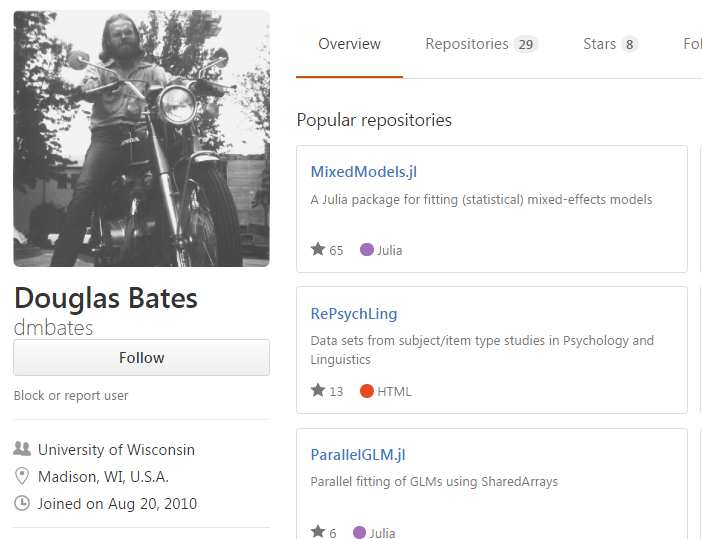
\includegraphics[width=0.97\linewidth]{images/douglasbatesgithub}
\end{figure}
\end{frame}	

\begin{frame}
	\frametitle{Statistics with Julia}
	\large
\texttt{MixedModels}
\begin{itemize}
\item development started in 2012 by Bates
\item little or no documentation outside of examples
\item implemented exclusively in Julia (about 1600 lines of code)
\item  fits LMMs.  Development of GLMM capabilities is planned.
\item single formula specification similar to lme4. 
\end{itemize}
\end{frame}
%============================================================%
\begin{frame}
	\frametitle{Statistics with Julia}
\large
\noindent \textbf{Douglas Bates on Mixed Models}\\ \medskip
	The most important aspect of Julia is "one
		language".  You develop in the same language in which you optimize.  \\
		\medskip
		The type system in Julia allows me to incorporate the different kinds of penalized least squares solvers in what to me is a clean way, thereby taking advantage of structural simplifications in simple, but common, cases. \\
		
		\medskip
		It is possible to do this in R/C++/Rcpp/EIgen but it would be a massive headache and perhaps beyond my abilities to do it well.

\end{frame}
%============================================================%
\begin{frame}
	\frametitle{Statistics with Julia}
	\large
\noindent \textbf{Douglas Bates on Mixed Models}\\ \medskip
The numerical methods implemented in lme4 are, in my opinion,
superior to those in nlme, mainly through the use of the relative
covariance factor and the profiled log-likelihood.  \\ \medskip

These may seem like details but to me they are very important.  The motiviation for
incorporating sparse matrix classes in the Matrix package and accessing the CHOLMOD code was to provide a general method for fitting such models.
\\ \medskip
Using C++, Rcpp and RcppEigen was motivated by trying to provide generality
and speed. The end result is confusing (my fault entirely) and fragile.

\end{frame}
%==============================================================%







\end{document}